\documentclass[14pt]{extbook}
\usepackage{multicol, enumerate, enumitem, hyperref, color, soul, setspace, parskip, fancyhdr} %General Packages
\usepackage{amssymb, amsthm, amsmath, bbm, latexsym, units, mathtools} %Math Packages
\everymath{\displaystyle} %All math in Display Style
% Packages with additional options
\usepackage[headsep=0.5cm,headheight=12pt, left=1 in,right= 1 in,top= 1 in,bottom= 1 in]{geometry}
\usepackage[usenames,dvipsnames]{xcolor}
\usepackage{dashrule}  % Package to use the command below to create lines between items
\newcommand{\litem}[1]{\item#1\hspace*{-1cm}\rule{\textwidth}{0.4pt}}
\pagestyle{fancy}
\lhead{Progress Quiz 3}
\chead{}
\rhead{Version A}
\lfoot{}
\cfoot{}
\rfoot{Fall 2020}
\begin{document}

\begin{enumerate}
\litem{
Solve the quadratic equation below. Then, choose the intervals that the solutions $x_1$ and $x_2$ belong to, with $x_1 \leq x_2$.\[ 25x^{2} +50 x + 24 = 0 \]\begin{enumerate}[label=\Alph*.]
\item \( x_1 \in [-1.25, -0.9] \text{ and } x_2 \in [-0.8, -0.72] \)
\item \( x_1 \in [-1.93, -1.43] \text{ and } x_2 \in [-0.61, -0.57] \)
\item \( x_1 \in [-30.05, -29.95] \text{ and } x_2 \in [-20.26, -19.88] \)
\item \( x_1 \in [-3.85, -3.47] \text{ and } x_2 \in [-0.29, -0.23] \)
\item \( x_1 \in [-6.09, -5.93] \text{ and } x_2 \in [-0.22, 0.09] \)

\end{enumerate} }
\litem{
Factor the quadratic below. Then, choose the intervals that contain the constants in the form $(ax+b)(cx+d); b \leq d.$\[ 54x^{2} -75 x + 25 \]\begin{enumerate}[label=\Alph*.]
\item \( a \in [0.4, 2.3], \hspace*{5mm} b \in [-46, -42], \hspace*{5mm} c \in [-0.9, 2.6], \text{ and } \hspace*{5mm} d \in [-32, -26] \)
\item \( a \in [16.5, 20.3], \hspace*{5mm} b \in [-9, -3], \hspace*{5mm} c \in [2.9, 3.3], \text{ and } \hspace*{5mm} d \in [-5, -1] \)
\item \( a \in [1.6, 4], \hspace*{5mm} b \in [-9, -3], \hspace*{5mm} c \in [13.3, 20], \text{ and } \hspace*{5mm} d \in [-5, -1] \)
\item \( a \in [8.1, 10.2], \hspace*{5mm} b \in [-9, -3], \hspace*{5mm} c \in [5.7, 6.9], \text{ and } \hspace*{5mm} d \in [-5, -1] \)
\item \( \text{None of the above.} \)

\end{enumerate} }
\litem{
Solve the quadratic equation below. Then, choose the intervals that the solutions belong to, with $x_1 \leq x_2$ (if they exist).\[ -15x^{2} -15 x + 3 = 0 \]\begin{enumerate}[label=\Alph*.]
\item \( x_1 \in [-1.19, -0.36] \text{ and } x_2 \in [-0.2, 0.3] \)
\item \( x_1 \in [-0.26, 0.53] \text{ and } x_2 \in [0.7, 2.1] \)
\item \( x_1 \in [-3.2, -2.33] \text{ and } x_2 \in [16.8, 17.9] \)
\item \( x_1 \in [-21.48, -20.04] \text{ and } x_2 \in [19.1, 20.1] \)
\item \( \text{There are no Real solutions.} \)

\end{enumerate} }
\litem{
Graph the equation below.\[ f(x) = -(x-1)^2 + 13 \]\begin{enumerate}[label=\Alph*.]
\begin{multicols}{2}\item 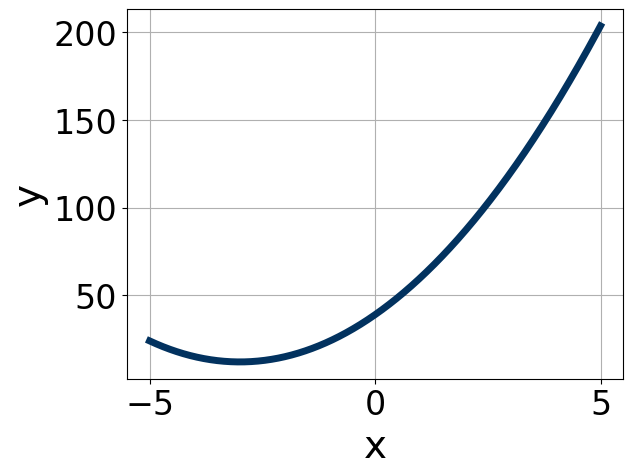
\includegraphics[width = 0.3\textwidth]{../Figures/quadraticEquationToGraphCopyAA.png}\item 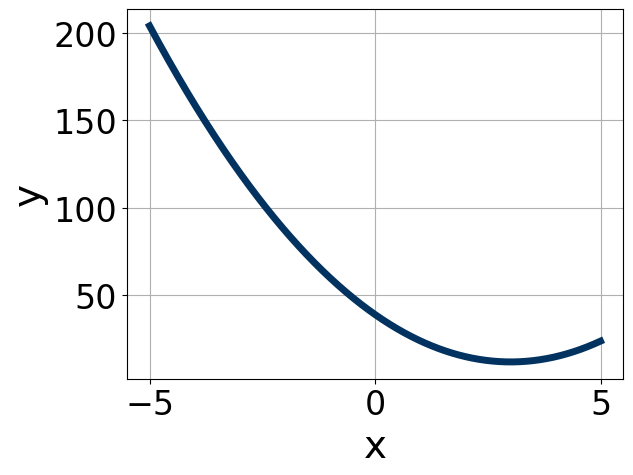
\includegraphics[width = 0.3\textwidth]{../Figures/quadraticEquationToGraphCopyBA.png}\item 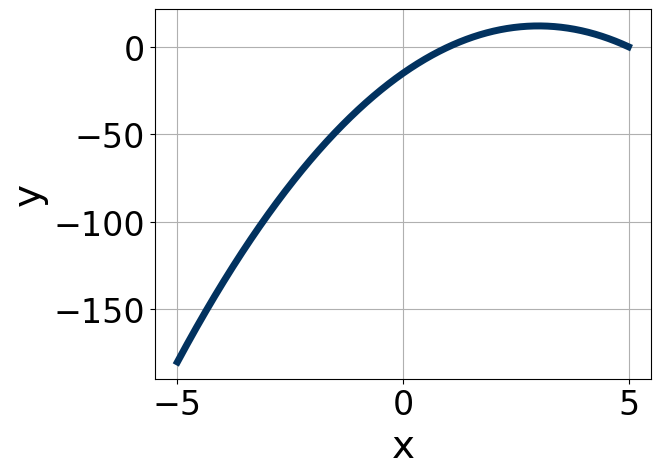
\includegraphics[width = 0.3\textwidth]{../Figures/quadraticEquationToGraphCopyCA.png}\item 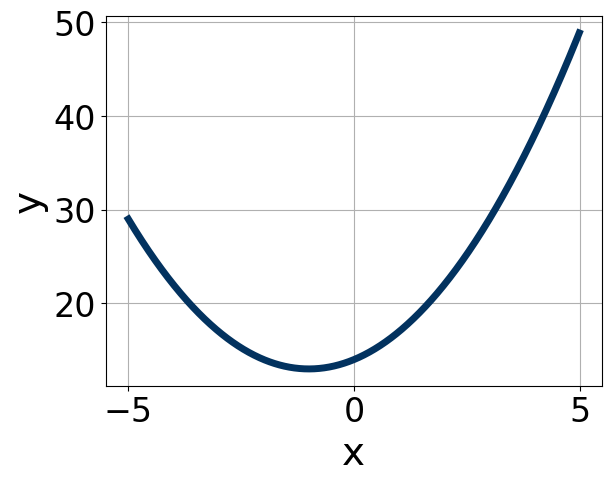
\includegraphics[width = 0.3\textwidth]{../Figures/quadraticEquationToGraphCopyDA.png}\end{multicols}\item None of the above.
\end{enumerate} }
\litem{
Solve the quadratic equation below. Then, choose the intervals that the solutions belong to, with $x_1 \leq x_2$ (if they exist).\[ -10x^{2} +9 x + 3 = 0 \]\begin{enumerate}[label=\Alph*.]
\item \( x_1 \in [-2.6, -0.4] \text{ and } x_2 \in [-0.47, 0.73] \)
\item \( x_1 \in [-1.1, 0.1] \text{ and } x_2 \in [1.04, 1.51] \)
\item \( x_1 \in [-12.2, -10.3] \text{ and } x_2 \in [1.76, 2.85] \)
\item \( x_1 \in [-14.9, -13.3] \text{ and } x_2 \in [14.42, 15.39] \)
\item \( \text{There are no Real solutions.} \)

\end{enumerate} }
\litem{
Graph the equation below.\[ f(x) = -(x+3)^2 + 16 \]\begin{enumerate}[label=\Alph*.]
\begin{multicols}{2}\item 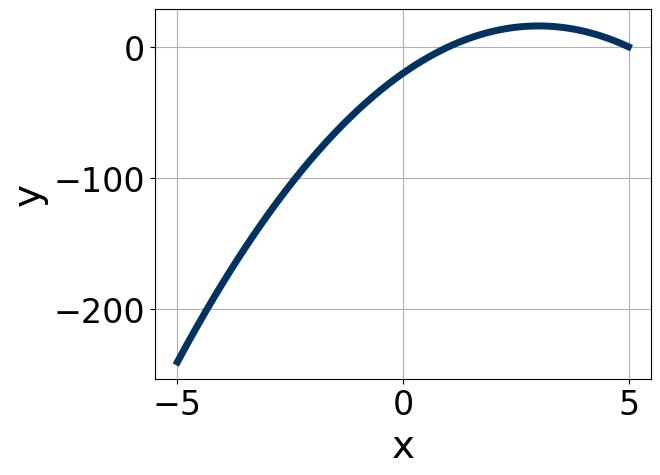
\includegraphics[width = 0.3\textwidth]{../Figures/quadraticEquationToGraphAA.png}\item 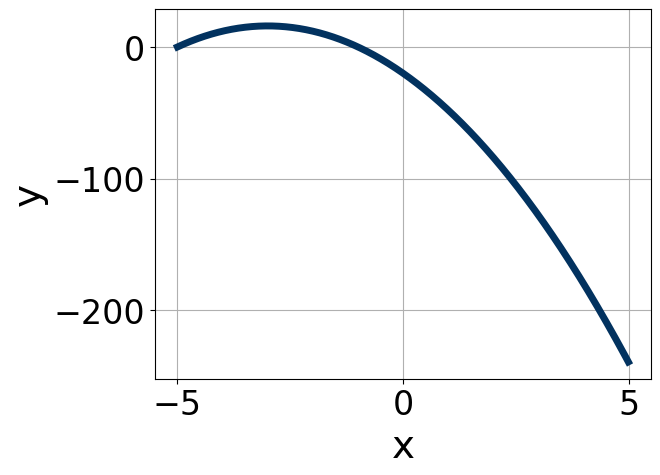
\includegraphics[width = 0.3\textwidth]{../Figures/quadraticEquationToGraphBA.png}\item 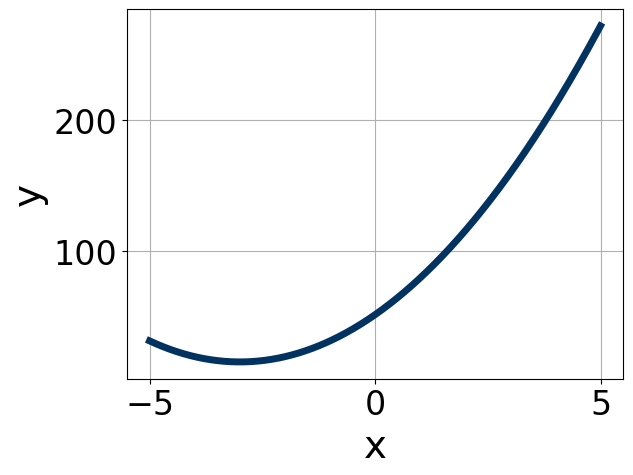
\includegraphics[width = 0.3\textwidth]{../Figures/quadraticEquationToGraphCA.png}\item 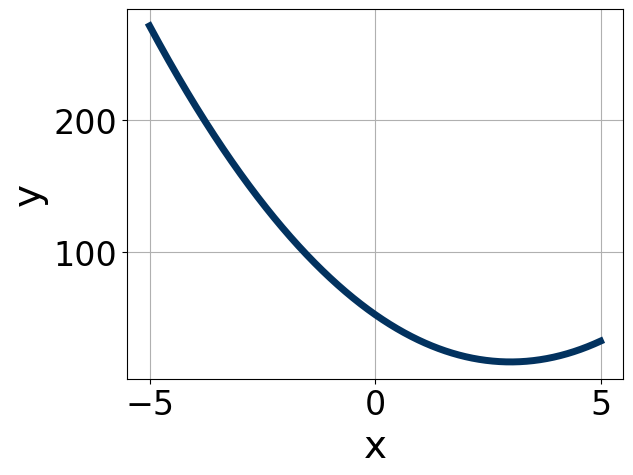
\includegraphics[width = 0.3\textwidth]{../Figures/quadraticEquationToGraphDA.png}\end{multicols}\item None of the above.
\end{enumerate} }
\litem{
Write the equation of the graph presented below in the form $f(x)=ax^2+bx+c$, assuming  $a=1$ or $a=-1$. Then, choose the intervals that $a, b,$ and $c$ belong to.
\begin{center}
    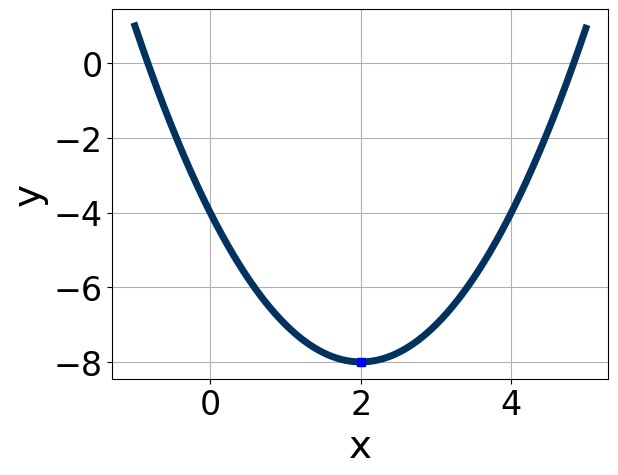
\includegraphics[width=0.5\textwidth]{../Figures/quadraticGraphToEquationA.png}
\end{center}
\begin{enumerate}[label=\Alph*.]
\item \( a \in [0.1, 1.1], \hspace*{5mm} b \in [1, 5], \text{ and } \hspace*{5mm} c \in [-5, -3] \)
\item \( a \in [0.1, 1.1], \hspace*{5mm} b \in [1, 5], \text{ and } \hspace*{5mm} c \in [12, 14] \)
\item \( a \in [-1.8, 0.5], \hspace*{5mm} b \in [-6, -1], \text{ and } \hspace*{5mm} c \in [-15, -10] \)
\item \( a \in [-1.8, 0.5], \hspace*{5mm} b \in [1, 5], \text{ and } \hspace*{5mm} c \in [-15, -10] \)
\item \( a \in [0.1, 1.1], \hspace*{5mm} b \in [-6, -1], \text{ and } \hspace*{5mm} c \in [-5, -3] \)

\end{enumerate} }
\litem{
Solve the quadratic equation below. Then, choose the intervals that the solutions $x_1$ and $x_2$ belong to, with $x_1 \leq x_2$.\[ 25x^{2} -60 x + 36 = 0 \]\begin{enumerate}[label=\Alph*.]
\item \( x_1 \in [0.45, 0.8] \text{ and } x_2 \in [2.38, 2.46] \)
\item \( x_1 \in [1.06, 1.39] \text{ and } x_2 \in [0.97, 1.68] \)
\item \( x_1 \in [29.92, 30.05] \text{ and } x_2 \in [29.7, 30.44] \)
\item \( x_1 \in [0.21, 0.25] \text{ and } x_2 \in [5.85, 6.2] \)
\item \( x_1 \in [0.35, 0.51] \text{ and } x_2 \in [3.22, 4.29] \)

\end{enumerate} }
\litem{
Write the equation of the graph presented below in the form $f(x)=ax^2+bx+c$, assuming  $a=1$ or $a=-1$. Then, choose the intervals that $a, b,$ and $c$ belong to.
\begin{center}
    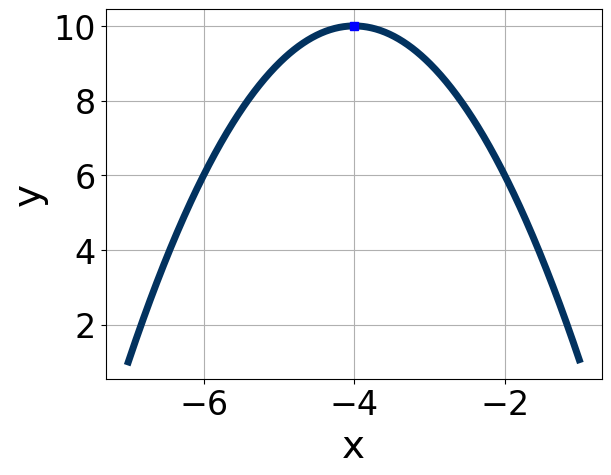
\includegraphics[width=0.5\textwidth]{../Figures/quadraticGraphToEquationCopyA.png}
\end{center}
\begin{enumerate}[label=\Alph*.]
\item \( a \in [-1.9, -0.6], \hspace*{5mm} b \in [7, 9], \text{ and } \hspace*{5mm} c \in [-30, -22] \)
\item \( a \in [-1.9, -0.6], \hspace*{5mm} b \in [-8, -6], \text{ and } \hspace*{5mm} c \in [-8, -5] \)
\item \( a \in [0.5, 2.5], \hspace*{5mm} b \in [7, 9], \text{ and } \hspace*{5mm} c \in [25, 27] \)
\item \( a \in [0.5, 2.5], \hspace*{5mm} b \in [-8, -6], \text{ and } \hspace*{5mm} c \in [25, 27] \)
\item \( a \in [-1.9, -0.6], \hspace*{5mm} b \in [7, 9], \text{ and } \hspace*{5mm} c \in [-8, -5] \)

\end{enumerate} }
\litem{
Factor the quadratic below. Then, choose the intervals that contain the constants in the form $(ax+b)(cx+d); b \leq d.$\[ 36x^{2} +60 x + 25 \]\begin{enumerate}[label=\Alph*.]
\item \( a \in [-0.58, 1.26], \hspace*{5mm} b \in [28, 33], \hspace*{5mm} c \in [-1.5, 1.4], \text{ and } \hspace*{5mm} d \in [24, 32] \)
\item \( a \in [2.92, 3.63], \hspace*{5mm} b \in [1, 10], \hspace*{5mm} c \in [11.4, 13.7], \text{ and } \hspace*{5mm} d \in [5, 10] \)
\item \( a \in [11.72, 12.59], \hspace*{5mm} b \in [1, 10], \hspace*{5mm} c \in [2.4, 3.8], \text{ and } \hspace*{5mm} d \in [5, 10] \)
\item \( a \in [5.97, 6.04], \hspace*{5mm} b \in [1, 10], \hspace*{5mm} c \in [5.3, 8.8], \text{ and } \hspace*{5mm} d \in [5, 10] \)
\item \( \text{None of the above.} \)

\end{enumerate} }
\end{enumerate}

\end{document}